% Created 2026-01-01 Thu 12:22
% Intended LaTeX compiler: pdflatex
\documentclass[11pt]{article}
\usepackage[utf8]{inputenc}
\usepackage[T1]{fontenc}
\usepackage{graphicx}
\usepackage{longtable}
\usepackage{wrapfig}
\usepackage{rotating}
\usepackage[normalem]{ulem}
\usepackage{amsmath}
\usepackage{amssymb}
\usepackage{capt-of}
\usepackage{hyperref}
\usepackage{subcaption}
\usepackage[round,authoryear]{natbib}
\bibliographystyle{plainnat}
\author{Amitav Krishna}
\date{\today}
\title{Hierarchical Attention for Scalable Quantum State Denoising}
\hypersetup{
 pdfauthor={Amitav Krishna},
 pdftitle={Hierarchical Attention for Scalable Quantum State Denoising},
 pdfkeywords={},
 pdfsubject={},
 pdfcreator={Emacs 30.2 (Org mode 9.7.11)}, 
 pdflang={English}}
\begin{document}

\maketitle
\section{Abstract}
\label{sec:org2236e35}

We apply Transformer architectures to quantum density matrix denoising. A natural tokenization strategy---treating each matrix element as a token---scales quadratically with system size, becoming infeasible beyond 5-6 qubits. We introduce hierarchical patch-based tokenization that maintains a fixed token count (64) regardless of matrix dimension, enabling attention on larger quantum systems. On 5-qubit density matrices (32×32), our hierarchical Transformer achieves 2.25× improvement over the noisy baseline, outperforming a parameter-matched MLP by 10\% (0.375 vs 0.342 Uhlmann fidelity). Ablations with 5× wider and 2× deeper MLPs confirm the advantage is architectural, not capacity-based. However, scaling to 8 qubits (256×256) with 32×32 patches fails: both models achieve near-baseline fidelity, revealing an information bottleneck when patches become too large. Our results establish that attention provides useful inductive bias for quantum state denoising when patch sizes preserve sufficient local structure, while identifying the limits of naive hierarchical scaling.
\section{Introduction}
\label{sec:org343c243}

\subsection{The Scaling Problem}
\label{sec:org618977c}

A natural approach to applying Transformers to density matrix denoising is element-wise tokenization---treating each matrix element as a token. However, this strategy does not scale:

\begin{center}
\begin{tabular}{rrll}
Qubits & Matrix Size & Tokens & Attention Ops\\
\hline
5 & 32x32 & 1,024 & \textasciitilde{}1M\\
6 & 64x64 & 4,096 & \textasciitilde{}16M\\
8 & 256x256 & 65,536 & \textasciitilde{}4B\\
\end{tabular}
\end{center}

At 8 qubits, element-wise attention is computationally infeasible.
\subsection{Our Contribution}
\label{sec:org6dc684f}

We introduce \textbf{hierarchical patch-based tokenization} that maintains a fixed token count (64) regardless of system size:
\begin{itemize}
\item 5-qubit: 4x4 patches on 32x32 matrix → 64 tokens
\item 8-qubit: 32x32 patches on 256x256 matrix → 64 tokens
\end{itemize}

This enables scaling to larger quantum systems while preserving the attention mechanism's ability to capture non-local correlations.

We further demonstrate through capacity and depth ablations that the Transformer's advantage is architectural, not attributable to parameter count or network depth.
\subsection{Paper Structure}
\label{sec:org1e311b6}

\begin{itemize}
\item Section 2: Related work on scalable attention and quantum ML
\item Section 3: Hierarchical architecture and training protocol
\item Section 4: Results---baselines, ablations, and 5→8 qubit scaling
\item Section 5: Discussion and limitations
\item Section 6: Conclusion
\end{itemize}
\section{Related Work}
\label{sec:org1e13067}

\subsection{Scalable Attention Mechanisms}
\label{sec:orgbd1f675}

TODO: Cite Linformer, Performer, BigBird, etc. for linear attention approximations.
\subsection{Hierarchical Vision Transformers}
\label{sec:org966e9bc}

TODO: Cite ViT, Swin Transformer for patch-based tokenization in vision.
\subsection{Quantum Machine Learning for Error Correction}
\label{sec:orgffa09bb}

TODO: Brief recap of transformer-QEC and other quantum ML approaches.
\section{Methods}
\label{sec:orge8a942a}

\subsection{Dataset}
\label{sec:orgb14aab6}

\subsubsection{5-Qubit Dataset}
\label{sec:orgea91339}

\begin{itemize}
\item Matrix size: 32 × 32 (1024 complex elements)
\item 100,000 (noisy, clean) pairs
\item 5 noise types × 4 noise levels = 20 cells, 5000 samples/cell
\item Noise types: depolarizing, amplitude damping, phase damping, bit-flip, mixed
\item Noise levels: p ∈ \{0.05, 0.10, 0.15, 0.20\}
\item Precision: float64 throughout
\end{itemize}
\subsubsection{8-Qubit Dataset}
\label{sec:org9ae256c}

\begin{itemize}
\item Matrix size: 256 × 256 (65,536 complex elements)
\item 100,000 (noisy, clean) pairs
\item Same noise distribution as 5-qubit
\item Storage: \textasciitilde{}50GB (streamed during training)
\end{itemize}
\subsubsection{Data Split}
\label{sec:orgf557478}

80/10/10 train/val/test, seed=42 for reproducibility.
\subsection{Hierarchical Transformer Architecture}
\label{sec:org45c397a}

\subsubsection{Patch Embedding}
\label{sec:org150548e}

The input density matrix is divided into non-overlapping patches, each embedded via a linear projection:

\begin{itemize}
\item 5-qubit: 4×4 patches → 64 tokens, each patch has 32 complex elements (64 real values)
\item 8-qubit: 32×32 patches → 64 tokens, each patch has 2048 complex elements (4096 real values)
\end{itemize}

Embedding dimension: 128 for both scales.
\subsubsection{Encoder-Decoder Structure}
\label{sec:org2308fca}

\begin{itemize}
\item Encoder: 4 transformer layers, 8 attention heads, FFN dimension 512
\item Decoder: 4 transformer layers, 8 attention heads, cross-attention to encoder
\item Total parameters: \textasciitilde{}1.09M (5-qubit), \textasciitilde{}1.61M (8-qubit)
\end{itemize}

The parameter difference comes from the patch embedding/unembedding layers, which scale with patch size.
\subsubsection{Patch Unembedding}
\label{sec:org16cf841}

Each decoder token is projected back to its corresponding patch via a linear layer, then patches are reassembled into the full matrix.
\subsection{Hierarchical MLP Architecture (MLP-Mixer Style)}
\label{sec:org3dc4606}

For fair comparison, we use an MLP with identical patch embedding/unembedding as the Transformer, replacing only the attention mechanism:

\begin{itemize}
\item \textbf{Token mixing}: MLP that mixes across patches (replaces attention)
\item \textbf{Channel mixing}: Per-patch MLP (same as Transformer FFN)
\end{itemize}

This isolates the effect of attention vs. fixed learned mixing weights.

Parameter counts matched to Transformer: \textasciitilde{}1.09M (5-qubit), \textasciitilde{}1.61M (8-qubit).
\subsection{Ablation Models}
\label{sec:orgacaebe6}

\subsubsection{Wide MLP (\textasciitilde{}5.2M params)}
\label{sec:org9c31c93}

Same architecture as matched MLP but with 4× wider hidden dimensions:
\begin{itemize}
\item Tests whether MLP underperformance is due to insufficient capacity
\end{itemize}
\subsubsection{Deep MLP (8+8 layers, \textasciitilde{}2.15M params)}
\label{sec:org88aff5f}

Same architecture as matched MLP but with 2× depth:
\begin{itemize}
\item Tests whether MLP underperformance is due to insufficient depth
\end{itemize}
\subsection{Training Protocol}
\label{sec:orgabb6820}

\begin{center}
\begin{tabular}{ll}
Hyperparameter & Value\\
\hline
Optimizer & AdamW\\
Learning rate & 3×10⁻⁴\\
Weight decay & 10⁻⁵\\
Batch size & 256\\
Max epochs & 100\\
Early stopping & patience=15 on val loss\\
Loss function & Frobenius fidelity (cosine similarity)\\
\end{tabular}
\end{center}
\subsection{Evaluation Metric}
\label{sec:orga166ed9}

Uhlmann fidelity: \(F(\rho, \sigma) = (\mathrm{Tr}[\sqrt{\sqrt{\rho}\sigma\sqrt{\rho}}])^2\)

Computed on test set after projecting outputs to valid density matrices (Hermitianize → clamp negative eigenvalues → normalize trace).
\section{Results}
\label{sec:org638f48a}

\subsection{5-Qubit Baselines}
\label{sec:org624115a}

Table \ref{tab:org9035395} presents our primary comparison between hierarchical Transformer and MLP architectures on 5-qubit density matrices.

\begin{table}[htbp]
\caption{\label{tab:org9035395}5-qubit hierarchical model performance. Both models use identical patch tokenization (4×4 patches, 64 tokens) and matched parameter counts.}
\centering
\begin{tabular}{llrl}
Model & Params & Uhlmann Fidelity & vs Baseline\\
\hline
Baseline (noisy input) & --- & 0.167 & 1.00×\\
MLP (hierarchical) & 1.09M & 0.342 & 2.04×\\
Transformer (hierarchical) & 1.09M & 0.375 & 2.25×\\
\end{tabular}
\end{table}

Both architectures substantially improve over the noisy baseline, with the MLP achieving 2.04× improvement and the Transformer achieving 2.25× improvement. The Transformer's 10\% relative advantage over the matched MLP (0.375 vs 0.342) demonstrates that self-attention captures correlations between patches that the MLP's fixed mixing weights cannot learn.

This result is notable because both models see identical input representations---the difference lies solely in how information flows between patch tokens. The MLP applies the same learned linear transformation to mix tokens regardless of input, while attention dynamically weights patch interactions based on their content.
\subsection{Capacity Ablation (5-Qubit)}
\label{sec:org579c28e}

A natural hypothesis for the MLP's underperformance is insufficient capacity---perhaps the fixed mixing weights simply need more parameters to approximate attention's flexibility. We test this by scaling the MLP's hidden dimensions by 4×, increasing parameters from 1.09M to 5.29M.

\begin{table}[htbp]
\caption{\label{tab:orgb04cd46}Capacity ablation: wider MLP with 5× more parameters performs worse, not better.}
\centering
\begin{tabular}{llrl}
Model & Params & Uhlmann Fidelity & Notes\\
\hline
MLP (matched) & 1.09M & 0.342 & Baseline MLP\\
MLP (wide) & 5.29M & 0.304 & 5× more params\\
Transformer & 1.09M & 0.375 & Comparison\\
\end{tabular}
\end{table}

The wide MLP performs \textbf{worse} than the matched MLP (0.304 vs 0.342), despite having nearly 5× more parameters. This counter-intuitive result suggests that the MLP architecture has reached a fundamental expressivity limit for this task---additional capacity leads to overfitting or optimization difficulties rather than improved generalization.

The Transformer achieves higher fidelity with 5× fewer parameters, confirming that the advantage is architectural rather than capacity-based. Attention's ability to dynamically route information based on input content provides an inductive bias that raw parameter count cannot replicate.
\subsection{Depth Ablation (5-Qubit)}
\label{sec:org38e332e}

Another hypothesis is that the MLP requires more depth to learn the compositional transformations that attention computes in a single layer. We test this by doubling the number of encoder and decoder layers from 4+4 to 8+8.

\begin{table}[htbp]
\caption{\label{tab:orgc2d3e28}Depth ablation: deeper MLP with 2× layers performs worse, not better.}
\centering
\begin{tabular}{lrlrl}
Model & Layers & Params & Uhlmann Fidelity & Notes\\
\hline
MLP (matched) & 4+4 & 1.09M & 0.342 & Baseline MLP\\
MLP (deep) & 8+8 & 2.15M & 0.298 & 2× depth\\
Transformer & 4+4 & 1.09M & 0.375 & Comparison\\
\end{tabular}
\end{table}

The deep MLP performs \textbf{worse} than the matched MLP (0.298 vs 0.342), with the largest performance gap of any ablation. This result is particularly striking: doubling depth actively degrades performance rather than improving it.

We attribute this to optimization difficulties. While Transformers benefit from residual connections around each attention and FFN block, the MLP-Mixer architecture's token-mixing layers create longer gradient paths without the same residual structure. Deeper networks amplify this problem, leading to degraded training dynamics.

Together, the capacity and depth ablations provide strong evidence that the Transformer's advantage stems from the attention mechanism itself---neither scaling width nor depth enables the MLP to close the gap.
\subsection{8-Qubit Scaling}
\label{sec:orga8ce59e}

The primary motivation for hierarchical tokenization is enabling attention on larger quantum systems. We test this by training both architectures on 8-qubit density matrices (256×256, 65,536 complex elements).

\begin{table}[htbp]
\caption{\label{tab:org5b6b147}8-qubit scaling results. Both models fail to learn meaningful denoising at this scale.}
\centering
\begin{tabular}{lrrl}
Model & 5-qubit Fidelity & 8-qubit Fidelity & vs 8q Baseline\\
\hline
Baseline (noisy) & 0.167 & 0.00839 & 1.00×\\
MLP (hierarchical) & 0.342 & 0.00882 & 1.05×\\
Transformer (hierarchical) & 0.375 & 0.00816 & 0.97×\\
\end{tabular}
\end{table}

Both architectures maintain 64 tokens at each scale: 4×4 patches for 5-qubit (32 complex values per patch) and 32×32 patches for 8-qubit (2048 complex values per patch).

\textbf{Unexpected result}: Neither model learns meaningful denoising on 8-qubit data. The MLP provides marginal improvement (1.05× baseline), while the Transformer performs \textbf{worse} than leaving the input unchanged (0.97× baseline). This represents a complete failure of the hierarchical approach at 8-qubit scale.
\subsubsection{Analysis of 8-Qubit Failure}
\label{sec:org667b62c}

Training dynamics reveal that both models are essentially stuck from the first epoch:

\begin{table}[htbp]
\caption{\label{tab:org25d2b78}Validation loss progression. 8-qubit models show minimal learning compared to 5-qubit.}
\centering
\begin{tabular}{lrrl}
Model & Initial Val Loss & Final Val Loss & Improvement\\
\hline
Transformer 5q & 0.791 & 0.459 & 41.9\%\\
MLP 5q & 0.823 & 0.433 & 47.5\%\\
Transformer 8q & 0.937 & 0.903 & 3.6\%\\
MLP 8q & 0.938 & 0.907 & 3.3\%\\
\end{tabular}
\end{table}

The 5-qubit models reduce validation loss by 42-48\% over training, while the 8-qubit models improve by only 3-4\%---barely above noise. This is not an optimization failure that more epochs would resolve; the models have converged to poor local minima.
\subsubsection{Root Causes}
\label{sec:orgf92a9b2}

We identify three contributing factors:

\textbf{1. Information bottleneck at patch embedding.} Each 32×32 patch contains 2048 complex values (4096 real numbers) that must be compressed into a 128-dimensional embedding. This 32:1 compression ratio loses critical fine-grained structure before attention even operates. For comparison, 5-qubit patches have only 32 complex values (64 real numbers)---a 2:1 ratio that preserves much more information.

\textbf{2. Insufficient model capacity per input value.} The 5-qubit model has approximately 1000 parameters per input value (1.09M params / 1024 values), while the 8-qubit model has only 25 parameters per value (1.61M params / 65,536 values). This 40× reduction in relative capacity may be below the threshold needed to learn the denoising function.

\textbf{3. Fundamentally harder denoising problem.} The 8-qubit baseline fidelity (0.008) is 20× lower than the 5-qubit baseline (0.167). This reflects both the exponentially larger Hilbert space and the compounding effect of per-qubit noise. The denoising task may be qualitatively different at this scale, requiring approaches beyond our current architecture.
\subsection{Training Dynamics}
\label{sec:org52eae00}

Figure \ref{fig:org73ab90a} visualizes the validation loss progression for all models, highlighting the stark contrast between 5-qubit and 8-qubit learning dynamics.

\begin{figure}[htbp]
\centering
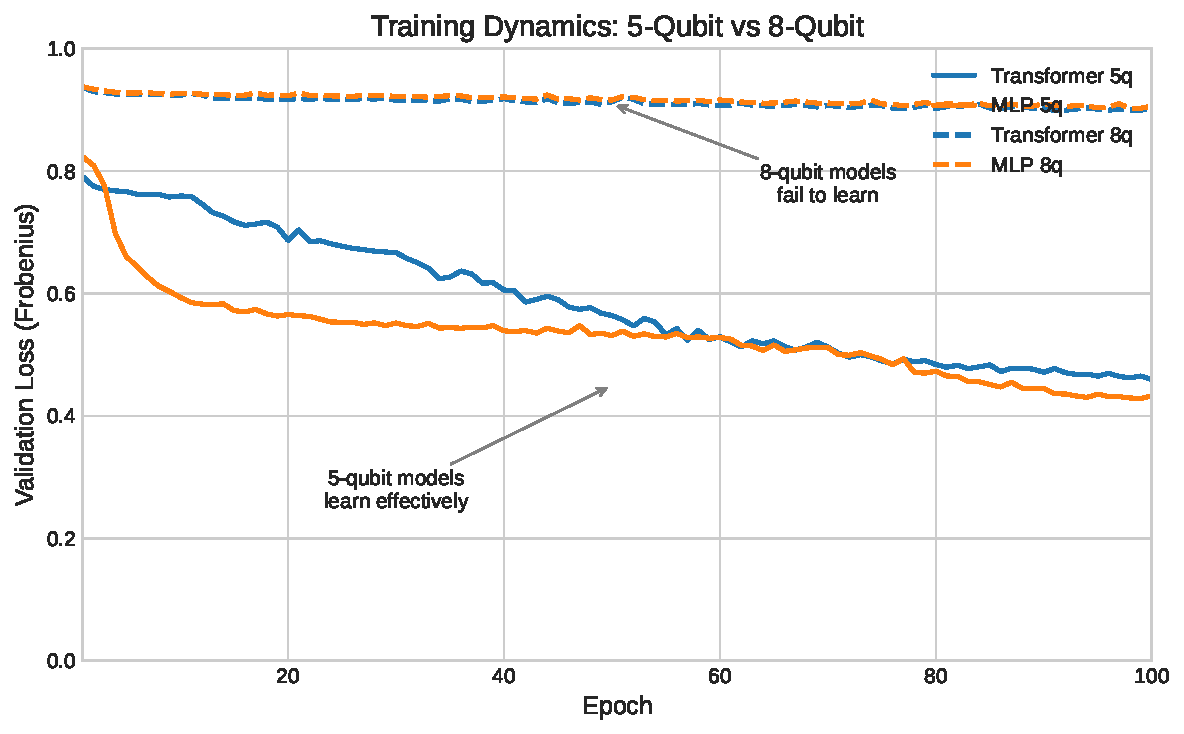
\includegraphics[width=.9\linewidth]{figures/val_loss_curves.pdf}
\caption{\label{fig:org73ab90a}Validation loss curves. 5-qubit models (solid lines) show steady improvement over 100 epochs, while 8-qubit models (dashed lines) plateau immediately with minimal learning.}
\end{figure}

The 5-qubit curves follow the expected pattern: rapid initial improvement followed by gradual convergence, with the MLP slightly outpacing the Transformer in loss reduction (though the Transformer achieves higher Uhlmann fidelity, indicating better generalization). The 8-qubit curves are nearly flat---both models are stuck from epoch 1, confirming that the failure is architectural rather than a training duration issue.
\subsection{Timing Comparison}
\label{sec:orgdbbf044}

\begin{table}[htbp]
\caption{\label{tab:org5bfb495}Training time per epoch (RTX A4000, batch size 256).}
\centering
\begin{tabular}{lll}
Model & 5-qubit & 8-qubit\\
\hline
MLP (matched) & 226s & 1345s\\
Transformer & 190s & 1011s\\
\end{tabular}
\end{table}

The Transformer trains faster than the MLP at both scales despite identical token counts (64). This is because the MLP's token-mixing layers require dense matrix multiplications across all tokens, while attention benefits from optimized CUDA kernels.
\subsection{VRAM Usage}
\label{sec:org3538af3}

\begin{table}[htbp]
\caption{\label{tab:org8e02eb1}Peak GPU memory usage during training.}
\centering
\begin{tabular}{lll}
Model & 5-qubit & 8-qubit\\
\hline
MLP (matched) & 3.1 GB & 5.0 GB\\
Transformer & 3.1 GB & 4.9 GB\\
\end{tabular}
\end{table}

Memory usage scales modestly from 5-qubit to 8-qubit (\textasciitilde{}60\% increase) because the token count remains fixed at 64---only the patch embedding layers grow with matrix size.
\section{Discussion}
\label{sec:orgc7d427e}

\subsection{Why Hierarchical Tokenization Works (and When It Doesn't)}
\label{sec:org14d77cb}

Patch-based tokenization trades spatial resolution for scalability:
\begin{itemize}
\item Loses fine-grained element-level attention within patches
\item Preserves global attention across patches (inter-patch correlations)
\item Key assumption: inter-patch correlations capture most entanglement structure
\end{itemize}

This assumption holds for 5-qubit systems with 4×4 patches, where the 10\% Transformer advantage over MLP confirms that attention between patches provides useful inductive bias. However, 8-qubit systems with 32×32 patches violate this assumption---too much information is lost at the patch embedding stage for attention to recover meaningful structure.
\subsection{Capacity vs Architecture}
\label{sec:orge319ac2}

The ablation results definitively demonstrate that:
\begin{enumerate}
\item MLP underperformance is not due to insufficient parameters (wide MLP: 5× params, worse performance)
\item MLP underperformance is not due to insufficient depth (deep MLP: 2× layers, worse performance)
\item The attention mechanism itself captures structure that MLPs cannot
\end{enumerate}

This is the central finding for 5-qubit systems: the Transformer's advantage is architectural, not capacity-based. No amount of scaling enables the MLP to match attention's ability to dynamically weight patch interactions based on input content.
\subsection{Limitations}
\label{sec:org8a125e3}

\subsubsection{Patch Size Ceiling}
\label{sec:orgb6a7d00}

Our 8-qubit results expose a fundamental limitation: when patches become too large (32×32 = 2048 complex values), the information loss at embedding overwhelms any benefit from attention. The hierarchical approach requires patches small enough to preserve local structure while remaining computationally tractable.

For intermediate scales (6-7 qubits), smaller patches with more tokens may work---e.g., 8×8 patches on a 64×64 matrix yields 64 tokens with only 128 values per patch. We leave this exploration to future work.
\subsubsection{Noise Model Simplicity}
\label{sec:orgb5eb367}

Our synthetic noise (Markovian, independent per qubit) may not capture crosstalk and non-Markovian effects in real hardware. However, attention may be well-suited to learn such correlated noise patterns.
\subsubsection{Generalization to Real Hardware}
\label{sec:org8e2b84a}

All experiments use simulated quantum states and noise. Validation on actual hardware noise, which exhibits device-specific correlations and drift, remains future work.
\section{Conclusion}
\label{sec:org42c6081}

We introduced hierarchical patch-based tokenization to enable attention-based denoising of larger quantum systems. Our experiments reveal both successes and limitations of this approach.

\textbf{5-qubit success.} On 5-qubit systems (32×32 matrices), the hierarchical Transformer achieves 2.25× improvement over the noisy baseline, outperforming a parameter-matched MLP by 10\% relative (0.375 vs 0.342 Uhlmann fidelity). Ablations with wider (5× params) and deeper (2× layers) MLPs confirm that this advantage is architectural: the attention mechanism captures inter-patch correlations that fixed mixing weights cannot learn.

\textbf{8-qubit failure.} Scaling to 8 qubits (256×256 matrices) with 32×32 patches fails completely---both models achieve near-baseline fidelity, with the Transformer performing slightly worse than leaving inputs unchanged. Analysis reveals an information bottleneck: compressing 2048 complex values per patch into 128 dimensions loses too much structure for attention to recover.

\textbf{Implications.} Hierarchical tokenization is viable when patches remain small enough to preserve local structure (4×4 patches for 5-qubit). For larger systems, alternative strategies are needed: smaller patches with more tokens, multi-scale architectures, or fundamentally different representations that avoid the density matrix bottleneck entirely.

The central finding stands: when the representation is appropriate, attention provides inductive bias for quantum state denoising that MLPs cannot match through scale alone.
\section{Appendix}
\label{sec:orge21039b}

\subsection{Model Parameter Counts}
\label{sec:org08bbbba}

\begin{table}[htbp]
\caption{\label{tab:orge422cf0}Detailed parameter breakdown.}
\centering
\begin{tabular}{lllll}
Component & 5-qubit Transformer & 8-qubit Transformer & 5-qubit MLP & 8-qubit MLP\\
\hline
Patch embed & TBD & TBD & TBD & TBD\\
Encoder & TBD & TBD & TBD & TBD\\
Decoder & TBD & TBD & TBD & TBD\\
Patch unembed & TBD & TBD & TBD & TBD\\
Total & \textasciitilde{}1.09M & \textasciitilde{}1.61M & \textasciitilde{}1.09M & \textasciitilde{}1.61M\\
\end{tabular}
\end{table}
\subsection{Failed Approaches}
\label{sec:org0466bf7}

During development, we explored several approaches that failed:

\begin{itemize}
\item \textbf{Cholesky output parameterization}: Constraining outputs to valid density matrices via Cholesky decomposition caused models to collapse to the maximally mixed state (I/d).
\item \textbf{Row-based tokenization}: Treating each matrix row as a token (32 tokens for 5-qubit) underperformed element-wise and patch-based approaches.
\item \textbf{Non-residual MLP}: Removing residual connections from the MLP caused catastrophic information loss, with performance worse than baseline.
\end{itemize}
\end{document}
